%!TEX root = ../thesis.tex
%*******************************************************************************
%*********************************** First Chapter *****************************
%*******************************************************************************

\chapter{Introduction}  %Title of the First Chapter

\ifpdf
    \graphicspath{{Chapter1/Figs/Raster/}{Chapter1/Figs/PDF/}{Chapter1/Figs/}}
\else
    \graphicspath{{Chapter1/Figs/Vector/}{Chapter1/Figs/}}
\fi


%********************************** %First Section  **************************************
\subsection{Hybrid Mappings}
Simulating quantum systems is one of the most promising applications of quantum computing in the near future~\cite{feynman2018simulating,lloyd1996universal,ortiz2002simulating}. The class of fermionic systems is particularly important and simulating them has an impressive range of applications: from problems in quantum chemistry~\cite{mcardle2020quantum,reiher2017elucidating}, to the Hubbard model in condensed matter physics~\cite{abrams1997simulation}, to Lattice Gauge Theories \cite{banuls2020simulating,chakraborty2022classically} and beyond. Classical methods applied to these problems do not scale favourably with the system size, whereas quantum techniques (e.g. VQE~\cite{mcclean2016theory}, Trotterization~\cite{tranter2019ordering} and others \cite{bravyi2002fermionic,friesner2005ab,ortiz2001quantum}) open up efficient avenues for studying static and dynamic properties of fermionic systems. In recent years, there has been a considerable experimental effort to simulate small fermionic systems on a quantum computer~\cite{barends2015digital,kokail2019self}.

 One of the crucial challenges facing these simulations is encoding the anti-commuting fermionic variables as operators acting on the qubit degrees of freedom. A desirable transformation would map interactions in the fermion picture to qubits resulting in (quasi-) local operators for the latter side. Furthermore, it should be engineered in a way to substantially reduce gate overhead in a circuit model -- leading to faster simulation times and more robustness with respect to errors.

There is currently no known fermion-to-qubit mapping that preserves perfect locality and consumes no auxiliary resources (in the form of qubits or the extra gate overhead) for an arbitrary interaction graph. However, in the last decade there has been remarkable progress towards designing efficient mappings~\cite{Verstraete_2005, 
setia2019superfast,havlivcek2017operator,bravyi2002fermionic,seeley2012bravyi, derby2021compact,chen2022equivalence, steudtner2019quantum} and exploring new ideas that would improve the existing ones~\cite{chiew2021optimal}. A summary of select mappings (including the most efficient ones) can be found in Table~\ref{tab:performance}. These mappings fall into two main categories: non-local mappings which require no additional resources but produce gate counts dependant on the total number of fermionic modes; local mappings which use additional resources (ancilla qubits) to produce constant gate counts independent of the number of fermionic modes. These local mappings can be physically interpreted as lattice gauge theories \cite{Chen_2018}. The best-known “explicitly constructed” local mapping is due to Chen and Xu~\cite{chen2022equivalence}. It uses the fewest qubits per fermion mode (1.25) while producing Hamiltonians with $k$-local average and maximum Pauli string, for constant $k$. There do exist general constructions with lower ratios that only require $1+ \frac{1}{k}$ qubits per fermion however they have the trade-off of a Pauli weight growing with $O(k)$. 

In this work, we introduce a family of parametrized Hybrid mappings (Section~\ref{section:Hybridmapping}) that combine the relaxed connectivity constraints of the Jordan-Wigner mapping and the increased locality of the Bravyi-Kitaev mapping to produce drastically reduced gate counts~\cite{tranter2018comparison}. In the context of limited qubit connectivity (Section~\ref{section:connectivity}) the Hybrid mapping produces gate counts that scale with $\frac{N}{2n}$ compared to $\frac{N}{2}$ for the Jordan-Wigner and Bravyi-Kitaev mappings on an $N\times N$ lattice (where $n \ll N$). In the regime of all-to-all connectivity the Hybrid mapping gate count scales with $\frac{N}{2n^2}$ (Section~\ref{section:hybridanalysis}) even further outperforming the unaffected Jordan-Wigner mapping. However, in the absence of connectivity constraints the Bravyi-Kitaev mapping gate count scales with $O(\log N)$. Despite this our numerical analysis in Section~\ref{section:numerical} shows the Hybrid mapping still results in lower gate counts than the Bravyi-Kitaev mapping for small lattices (e.g. lattices smaller than $164 \times 164$ for $n=4$).

We also construct a Hybrid\+ family of parametrized local mappings (Section~\ref{section:auxHybridmapping}) which only require $1+\frac{1}{n^2}$ qubits per fermionic mode. Our construction interpolates between the Auxillary Qubit mapping~\cite{Verstraete_2005, steudtner2019quantum} and the Bravyi-Kitaev mapping by setting $n=1$ for the former and $n=N$ for the latter. For all the intermediate $n$, our construction results in novel highly efficient mappings that produce a dramatic reduction in the number of auxiliary qubits required, while simultaneously generating local Pauli strings. We illustrate examples for $n=4$ and $n=8$ which demonstrate 1.0625 and 1.0156 qubit-to-fermion ratios compared to the best existing local mapping \cite{chen2022equivalence} which achieves a 1.25 qubit-to-fermion ratio.

The key insight of our work is that it is possible to apply seemly incompatible mappings on different scales such that their relative strengths complement each other. We combine the efficiency of the Bravyi-Kitaev mapping with the low connectivity restraints of the Jordan-Wigner mapping to produce a far superior Hybrid mapping. On a small scale (within each cell) we use the Bravyi-Kitaev mapping (in few fermion regime when it's connectivity restraints are not too large), but when we zoom out to a larger scale we use the Jordan-Wigner mapping between the cells. By varying the scale at which each mapping is dominant we are able to find an optimal mapping for a given quantum computer. 


\section{Preliminaries}
 In this section, we introduce the mappings our Hybrid schemes extend: the Jordan-Wigner Mapping (Section~\ref{section:jordan-wigner}), the Bravyi-Kitaev Mapping (Section~\ref{section:bravyi-kitaev}), and the Auxiliary Qubit Mapping (Section~\ref{section:auxillaryMappings}).

\subsection{Jordan-Wigner Mapping}
\label{section:jordan-wigner}
The Jordan-Wigner transform \cite{jordan1993paulische} is arguably the oldest known fermion-to-qubit mapping. It stores the occupation number of the $i$-th fermionic mode in the $i$-th qubit. Therefore, all the non-local behaviour (the parity information) has to be encoded in the operators \cite{chiew2021optimal}:
\begin{align}
        a_i \rightarrow \left( \bigotimes_{k=1}^{i-1} Z_k \right) \sigma_i^-\\
        a^{\dagger}_i \rightarrow \left( \bigotimes_{k=1}^{i-1} Z_k \right) \sigma_i^+
\end{align}
where
\begin{align}
        \sigma^-_i = \frac{1}{2} (X_i + i Y_i) = \ket{0}_i \bra{1}_i\\
        \sigma^+_i = \frac{1}{2} (X_i - i Y_i) = \ket{1}_i \bra{0}_i 
\end{align}
The $\bigotimes_{k=1}^{i-1} Z_k$ term is necessary to apply the parity phase shift $(-1)^{\sum_{k=0}^{i-1} f_k}$, where $f_k$ are defined below. These operators act in exactly the same way on a qubit spin basis as the fermionic creation and annihilation operators act upon the Fock basis in Eqns~\eqref{secondQuant1} and~\eqref{secondQuant2}.

\begin{equation}
    \label{secondQuant1}
    a_p \ket{f_0,\cdots, f_i, \cdots, f_{M-1}} = \delta_{f_p, 1} (-1)^{\sum_{i=0}^{p-1} f_i} \ket{f_0,\cdots, f_p \oplus 1, \cdots, f_{M-1}}
    \end{equation}
\begin{equation}
    \label{secondQuant2}
    a_p^{\dagger} \ket{f_0,\cdots, f_i, \cdots, f_{M-1}} = \delta_{f_p, 0} (-1)^{\sum_{i=0}^{p-1} f_i}
    \ket{f_0,\cdots, f_p \oplus 1, \cdots, f_{M-1}}
    \end{equation}
\subsection{Bravyi-Kitaev Mapping}
\label{section:bravyi-kitaev}
Our construction may be regarded as a particular extension of the Bravyi-Kitaev mapping \cite{Bravyi_2002}. Previous extensions of the Bravyi-Kitaev mapping have combined the Bravyi-Kitaev fast and super-fast mappings to logarithmically reduce the Pauli weight of fermionic operators \cite{Setia_2019}.

The Bravyi-Kitaev mapping stores the parity of fermionic modes in a non-local Fenwick tree data structure \cite{havlivcek2017operator}. A Fenwick tree \cite{fenwick1994new} is a partial ordering of binary representations where every node is a copy of its parent with one of the $1$s changed to a $0$ as shown in Figure~\ref{fenwick_trees}. In this section we outline how the Bravyi-Kitaev mapping encodes $m$ fermionic modes:

First, each fermionic mode is assigned a corresponding qubit and a node in a Fenwick tree. Every qubit stores the total parity of the fermionic modes below it in the Fenwick tree. This allows fermionic operators to be constructed with Pauli-weight $O(\log m)$.

These operators (as shown in~\cite{seeley2012bravyi}) are constructed using three easily calculated subsets of the Fenwick tree: the Update ($U$), Parity ($P$), and Flip ($F$)  sets.
\begin{dmath*}
a_i \rightarrow X_{U_i}  \sigma^-_i  Z_{ P_i/F_i} \rightarrow \frac{1}{2}\left( \bigotimes_{j \in U_i} X_j \otimes X_i \otimes \bigotimes_{j \in P_i} Z_j + i \bigotimes_{j \in U_i} X_j \otimes Y_i\otimes \bigotimes_{j \in P_i/F_i} Z_j \right)
\end{dmath*}
\begin{dmath*}
a^{\dagger}_i \rightarrow X_{U_i}  \sigma^+_iZ_{ P_i/F_i} \rightarrow \frac{1}{2}\left( \bigotimes_{j \in U_i} X_j \otimes X_i \otimes \bigotimes_{j \in P_i} Z_j - i \bigotimes_{j \in U_i} X_j \otimes Y_i\otimes \bigotimes_{j \in  P_i/F_i} Z_j \right) 
\end{dmath*}
Each of the above sets is defined (similarly to the original formulation \cite{seeley2012bravyi}) as follows :

Use the binary representation: $\alpha = \alpha_{l-1}\ldots \alpha_0$ and $\beta = \beta_{l-1}\ldots \beta_0$, where index $0$ denotes the most significant bit. Define $\prec$ to represent the partial ordering of the Fenwick tree. Fermionic modes are zero-indexed.

\begin{definition} Let the Update Set $U(\alpha)$ be such that $\beta \in U(\alpha)$ if and only if for some $i_0$, $\alpha_{i_0} = 0$ and $\alpha_i = \beta_i$ for $i\geq i_0$ and $\beta_i = 1$ for $i \leq i_0$. Equivalent to $\beta \in U(\alpha)$ if and only if $\alpha \prec \beta$.
\end{definition}

\begin{definition} Let the Parity set $P(\alpha)$ contain elements $\beta \in P(\alpha)$ if and only if for some $i_0$: $\alpha_{i_0} = 1$, $\beta_{i_0} = 0$, $\beta_i = \alpha_i$ for $i> i_0$ and $\beta_i = 1$ for $i< i_0$, then $
        \sum_{j \in P(i)} q_j = \sum_{j < i} f_j$
\end{definition}

\begin{definition} Let the Flip set $F(\alpha)$ contain elements $\beta \in F(\alpha)$ if and only if for some $i_0$: $\beta_{i_0} = 0$, $\beta_i = \alpha_i$ for $i\neq i_0$ and $\alpha_i = 1$ for $i\leq i_0$, then $
 \sum_{j \in F(i)} q_j = \sum_{j \prec i} f_j$
\end{definition}

Examples of these sets are given in Figure~\ref{fenwick_trees}. We present three simple algorithms for generating these sets which will later be used in our construction: \hyperref[GenerateUpdateSet]{\textsc{GenerateUpdateSet}}, \hyperref[GenerateParitySet]{\textsc{GenerateParitySet}}, and \hyperref[GenerateFlipSet]{\textsc{GenerateFlipSet}}.
\begin{figure}[htbp]
  \centering
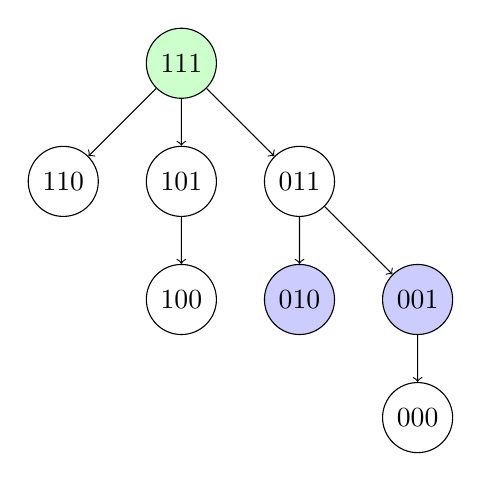
\begin{tikzpicture}[nodes={draw, circle}, ->]
        \node[fill = green!20]{111}
                child{node {110}}
                child{node {101}
                        child{ node{100} }
                }
                child{node {011}
                        child [missing]
                        child{node[fill = blue!20]{010}}
                        child{node[fill = blue!20]{001} 
                                child{node{000}}
                        }
                };
\end{tikzpicture}
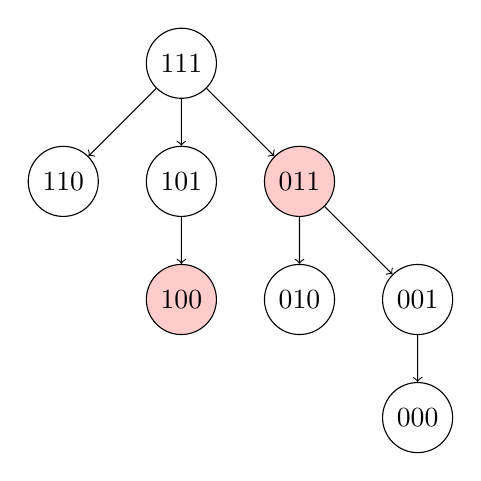
\begin{tikzpicture}[nodes={draw, circle}, ->]
        \node{111}
                child{node{110}}
                child{node {101}
                        child{ node[fill= red!20]{100} }
                }
                child{node[fill = red!20] {011}
                        child [missing]
                        child{node{010}}
                        child{node{001} 
                                child{node{000}}
                        }
                };
\end{tikzpicture}
\caption{\label{fenwick_trees} \textbf{Top:}  Update set (green) and Flip set (blue) for $i=3$ $(011)$ on Fenwick tree with $N=8$. \textbf{Bottom:} Parity set (red) for $i=5$ $(101)$ on Fenwick tree with $N=8$.}
\end{figure} \noindent

\begin{algorithm}[htbp]
\caption{\textsc{GenerateUpdateSet}\label{GenerateUpdateSet}}
\begin{algorithmic}[1]
\Require{Fermionic enumeration: $\alpha$, Number of fermionic modes: $n$}
\Ensure{Update Set $U_{\alpha}$}
\State updateSet = \{\}
\State $l \gets $ length of binary representation of $\alpha$
\State $\beta \gets \alpha$
\For{$i$ counting from $0$ to $l-1$}
    \If{$\alpha_i$ is $0$}
        \State $\beta \gets \beta_{l-1}\ldots\beta_{i+1}1\beta_{i-1}\ldots\beta_0$
        \If{$\beta < n$}
            \State Add $\beta$ to updateSet
        \EndIf
    \EndIf
\EndFor

\end{algorithmic}
\end{algorithm}

\begin{algorithm}[htbp]
    \caption{\label{GenerateParitySet}\textsc{GenerateParitySet}}
\begin{algorithmic}[1]
\Require{Fermionic enumeration: $\alpha$}
\Ensure{Parity Set $P_{\alpha}$}
\State paritySet = \{\}
\State $l \gets $ length of binary representation of $\alpha$
\For{$i$ counting down from $l-1$ to $0$}
    \If{$\alpha_i$ is $1$}
        \State $\beta \gets \alpha_{l-1}\alpha_{l-2}\ldots\alpha_{i+1}01\ldots 1$
        \State Add $\beta$ to paritySet 
    \EndIf
\EndFor
\end{algorithmic}
\end{algorithm}
\begin{algorithm}[htbp]
    \caption{\label{GenerateFlipSet}\textsc{GenerateFlipSet}}
\begin{algorithmic}[1]
\Require{Fermionic enumeration: $\alpha$}
\Ensure{Flip Set $F_{\alpha}$}
\State flipSet = \{\}
\State $l \gets $ length of binary representation of $\alpha$
\State $i \gets 0$
\While{$\alpha_i$ is $1$}
    \State $\beta \gets \alpha_{l-1}\ldots \alpha_{i+1}0\alpha_{i-1} \ldots \alpha_0$
    \State Add $\beta$ to flipSet
    \State $i \gets i + 1$
\EndWhile
\end{algorithmic}
\end{algorithm}

\subsection{Auxiliary Qubit Mapping}
\label{section:auxillaryMappings}
Though originally pioneered by \cite{Verstraete_2005}, here we recall the formalization of the auxiliary mappings from~\cite{steudtner2019quantum}. The principle behind auxiliary mapping schemes is to create stabilisers which are similar to non-local interaction terms in the Hamiltonian, so they can be used to cancel each other out. For example, consider an $n$-qubit Hamiltonian consisting of $m$ Pauli-strings $h_i$ some of which contain a non-local Pauli-string $p$:
\begin{equation}
    H = \sum_{i=0}^m h_i
\end{equation}
\begin{itemize}
\item Let $\ket{\psi}_S$ be an arbitrary state on the $n$-qubit system ($\mathcal{H}_S$)
\item Introduce an ancillary qubit $\ket{0}_A$ ($\mathcal{H}_A$)
\item Entangle the ancilla with the $n$-qubit state by applying a given unitary $V$
\begin{equation}
    V \ket{\psi}_S \ket{0}_A = \ket{\tilde \psi}_{SA}
\end{equation}
\item Find $\sigma$ such that $(p \otimes \sigma)$ is a stabiliser:
\begin{equation}
    (p \otimes \sigma) \ket{\tilde \psi}_{SA} = \ket{\tilde \psi}_{SA}
\end{equation}
\item Modify $H$ so it commutes with the stabiliser (\ref{eq:commute_with_hamiltonian}) and thus acting with the modified Hamiltonian $\tilde H$ on a stabiliser state always produces another stabiliser state. This involves adding an operator $\kappa$ to each term $h_i$ in the Hamiltonian that anti-commutes with $(p \otimes \sigma)$ to produce a commuting term $h_i^{(\kappa)} = h_i \otimes \kappa$. This modification must be such that its action on the entangled system is equivalent to the action of the original Hamiltonian on the $n$-qubit state (\ref{eq:equivalent_to_original_hamiltonian}).
\begin{equation}
\label{eq:commute_with_hamiltonian}
    H^{(\kappa)}(p \otimes \sigma)  \ket{\tilde \psi}_{SA} =(p \otimes \sigma)  H^{(\kappa)}\ket{\tilde \psi}_{SA}  
\end{equation}
\begin{equation}
    \label{eq:equivalent_to_original_hamiltonian}
    H^{(\kappa)}\ket{\tilde \psi}_{SA} = V (H \otimes I) \ket{\psi}_S \ket{0}_A
\end{equation}
\item Now we can use the stabiliser to cancel out the non-local $p$ string in the Hamiltonian to get a simplified Hamiltonian $\tilde H$ which is logically identical.
\begin{equation}
   \tilde h_i = \begin{cases} h_i^{(\kappa)} (p \otimes \sigma)  &  p \in h_i \\ 
   h_i^{(\kappa)} & p \notin h_i \end{cases}
\end{equation}
\begin{equation}
    \tilde H = \sum_{i=0}^m \tilde h_i
\end{equation}
\end{itemize}
To perform this procedure to remove multiple non-local strings $p_i$, we can simply repeat the process with additional ancillas. However as the stabilisers $p_i \otimes \sigma_i$ must share common stabiliser states, it is only possible to simultaneously remove commuting strings. 
